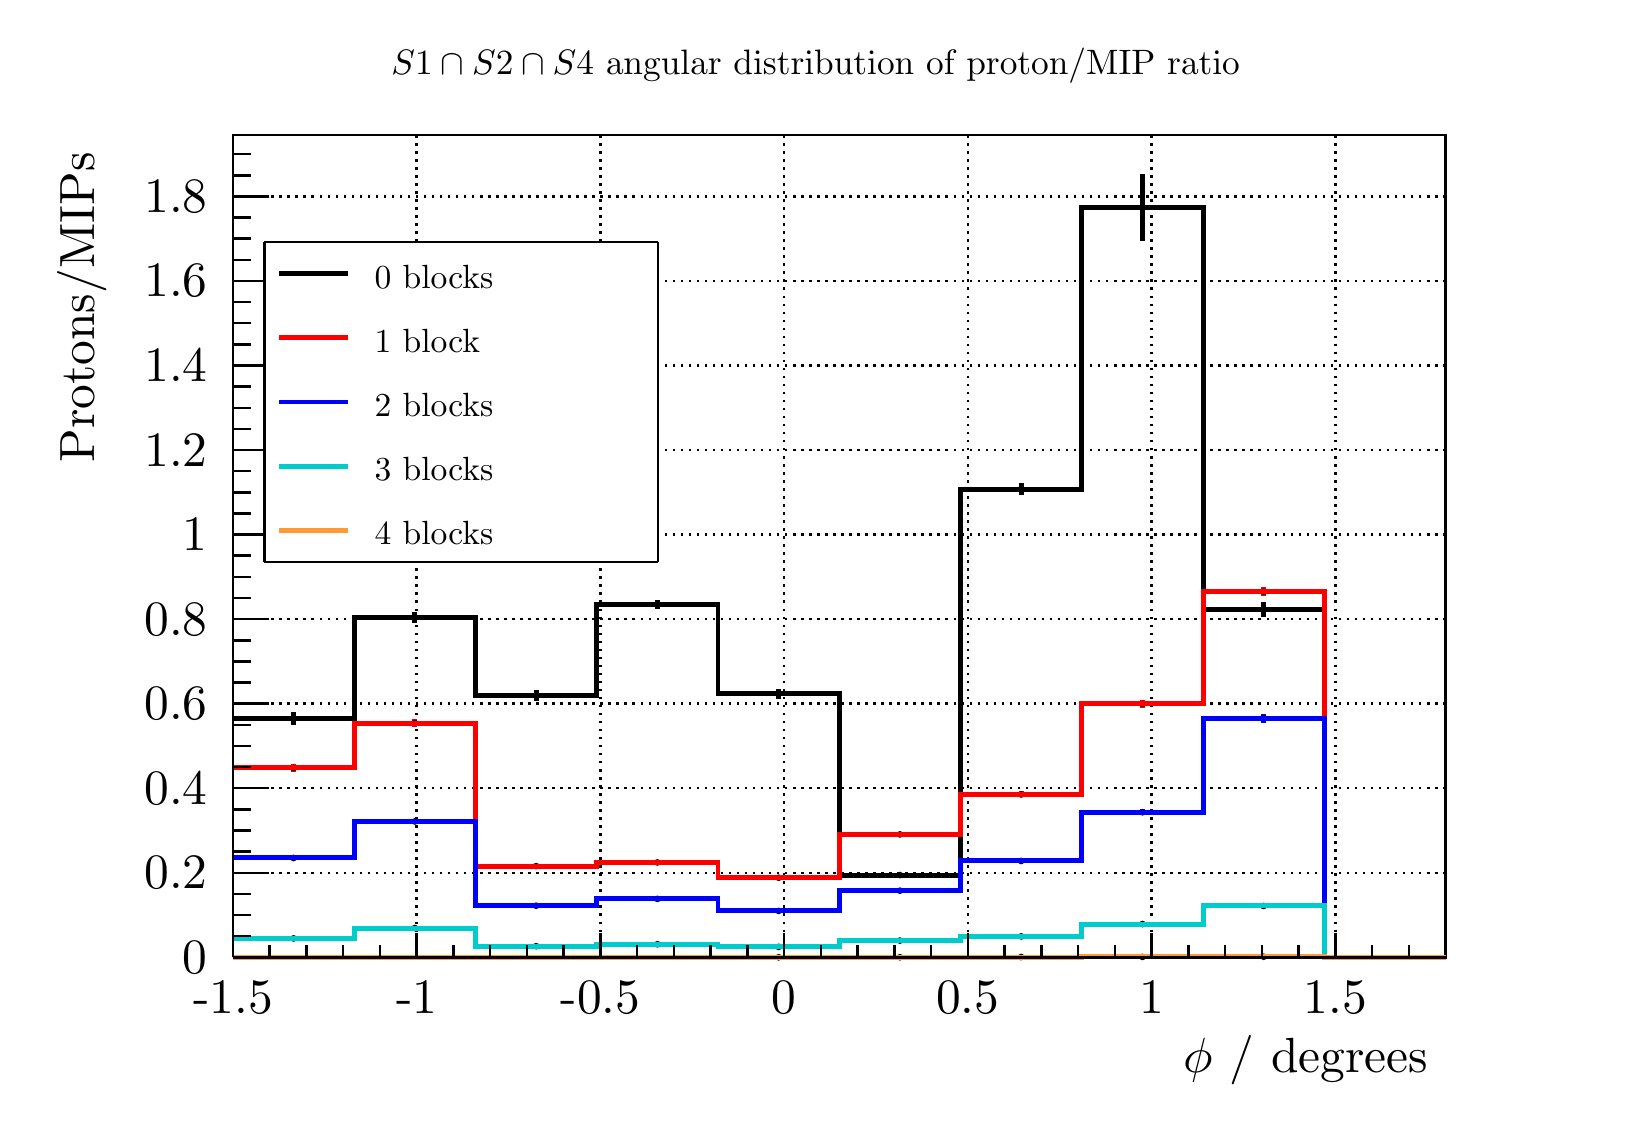
\begin{tikzpicture}
\pgfdeclareplotmark{cross} {
\pgfpathmoveto{\pgfpoint{-0.3\pgfplotmarksize}{\pgfplotmarksize}}
\pgfpathlineto{\pgfpoint{+0.3\pgfplotmarksize}{\pgfplotmarksize}}
\pgfpathlineto{\pgfpoint{+0.3\pgfplotmarksize}{0.3\pgfplotmarksize}}
\pgfpathlineto{\pgfpoint{+1\pgfplotmarksize}{0.3\pgfplotmarksize}}
\pgfpathlineto{\pgfpoint{+1\pgfplotmarksize}{-0.3\pgfplotmarksize}}
\pgfpathlineto{\pgfpoint{+0.3\pgfplotmarksize}{-0.3\pgfplotmarksize}}
\pgfpathlineto{\pgfpoint{+0.3\pgfplotmarksize}{-1.\pgfplotmarksize}}
\pgfpathlineto{\pgfpoint{-0.3\pgfplotmarksize}{-1.\pgfplotmarksize}}
\pgfpathlineto{\pgfpoint{-0.3\pgfplotmarksize}{-0.3\pgfplotmarksize}}
\pgfpathlineto{\pgfpoint{-1.\pgfplotmarksize}{-0.3\pgfplotmarksize}}
\pgfpathlineto{\pgfpoint{-1.\pgfplotmarksize}{0.3\pgfplotmarksize}}
\pgfpathlineto{\pgfpoint{-0.3\pgfplotmarksize}{0.3\pgfplotmarksize}}
\pgfpathclose
\pgfusepathqstroke
}
\pgfdeclareplotmark{cross*} {
\pgfpathmoveto{\pgfpoint{-0.3\pgfplotmarksize}{\pgfplotmarksize}}
\pgfpathlineto{\pgfpoint{+0.3\pgfplotmarksize}{\pgfplotmarksize}}
\pgfpathlineto{\pgfpoint{+0.3\pgfplotmarksize}{0.3\pgfplotmarksize}}
\pgfpathlineto{\pgfpoint{+1\pgfplotmarksize}{0.3\pgfplotmarksize}}
\pgfpathlineto{\pgfpoint{+1\pgfplotmarksize}{-0.3\pgfplotmarksize}}
\pgfpathlineto{\pgfpoint{+0.3\pgfplotmarksize}{-0.3\pgfplotmarksize}}
\pgfpathlineto{\pgfpoint{+0.3\pgfplotmarksize}{-1.\pgfplotmarksize}}
\pgfpathlineto{\pgfpoint{-0.3\pgfplotmarksize}{-1.\pgfplotmarksize}}
\pgfpathlineto{\pgfpoint{-0.3\pgfplotmarksize}{-0.3\pgfplotmarksize}}
\pgfpathlineto{\pgfpoint{-1.\pgfplotmarksize}{-0.3\pgfplotmarksize}}
\pgfpathlineto{\pgfpoint{-1.\pgfplotmarksize}{0.3\pgfplotmarksize}}
\pgfpathlineto{\pgfpoint{-0.3\pgfplotmarksize}{0.3\pgfplotmarksize}}
\pgfpathclose
\pgfusepathqfillstroke
}
\pgfdeclareplotmark{newstar} {
\pgfpathmoveto{\pgfqpoint{0pt}{\pgfplotmarksize}}
\pgfpathlineto{\pgfqpointpolar{44}{0.5\pgfplotmarksize}}
\pgfpathlineto{\pgfqpointpolar{18}{\pgfplotmarksize}}
\pgfpathlineto{\pgfqpointpolar{-20}{0.5\pgfplotmarksize}}
\pgfpathlineto{\pgfqpointpolar{-54}{\pgfplotmarksize}}
\pgfpathlineto{\pgfqpointpolar{-90}{0.5\pgfplotmarksize}}
\pgfpathlineto{\pgfqpointpolar{234}{\pgfplotmarksize}}
\pgfpathlineto{\pgfqpointpolar{198}{0.5\pgfplotmarksize}}
\pgfpathlineto{\pgfqpointpolar{162}{\pgfplotmarksize}}
\pgfpathlineto{\pgfqpointpolar{134}{0.5\pgfplotmarksize}}
\pgfpathclose
\pgfusepathqstroke
}
\pgfdeclareplotmark{newstar*} {
\pgfpathmoveto{\pgfqpoint{0pt}{\pgfplotmarksize}}
\pgfpathlineto{\pgfqpointpolar{44}{0.5\pgfplotmarksize}}
\pgfpathlineto{\pgfqpointpolar{18}{\pgfplotmarksize}}
\pgfpathlineto{\pgfqpointpolar{-20}{0.5\pgfplotmarksize}}
\pgfpathlineto{\pgfqpointpolar{-54}{\pgfplotmarksize}}
\pgfpathlineto{\pgfqpointpolar{-90}{0.5\pgfplotmarksize}}
\pgfpathlineto{\pgfqpointpolar{234}{\pgfplotmarksize}}
\pgfpathlineto{\pgfqpointpolar{198}{0.5\pgfplotmarksize}}
\pgfpathlineto{\pgfqpointpolar{162}{\pgfplotmarksize}}
\pgfpathlineto{\pgfqpointpolar{134}{0.5\pgfplotmarksize}}
\pgfpathclose
\pgfusepathqfillstroke
}
\definecolor{c}{rgb}{1,1,1};
\draw [color=c, fill=c] (0,0) rectangle (20,13.5632);
\draw [color=c, fill=c] (2.6,1.76322) rectangle (18,12.2069);
\definecolor{c}{rgb}{0,0,0};
\draw [c,line width=0.9] (2.6,1.76322) -- (2.6,12.2069) -- (18,12.2069) -- (18,1.76322) -- (2.6,1.76322);
\definecolor{c}{rgb}{1,1,1};
\draw [color=c, fill=c] (2.6,1.76322) rectangle (18,12.2069);
\definecolor{c}{rgb}{0,0,0};
\draw [c,line width=0.9] (2.6,1.76322) -- (2.6,12.2069) -- (18,12.2069) -- (18,1.76322) -- (2.6,1.76322);
\draw [c,line width=0.9] (2.6,1.76322) -- (18,1.76322);
\draw [c,dotted,line width=0.9] (2.6,12.2069) -- (2.6,1.76322);
\draw [c,dotted,line width=0.9] (4.93333,12.2069) -- (4.93333,1.76322);
\draw [c,dotted,line width=0.9] (7.26667,12.2069) -- (7.26667,1.76322);
\draw [c,dotted,line width=0.9] (9.6,12.2069) -- (9.6,1.76322);
\draw [c,dotted,line width=0.9] (11.9333,12.2069) -- (11.9333,1.76322);
\draw [c,dotted,line width=0.9] (14.2667,12.2069) -- (14.2667,1.76322);
\draw [c,dotted,line width=0.9] (16.6,12.2069) -- (16.6,1.76322);
\draw [c,dotted,line width=0.9] (16.6,12.2069) -- (16.6,1.76322);
\draw [c,line width=0.9] (2.6,1.76322) -- (2.6,12.2069);
\draw [c,dotted,line width=0.9] (18,1.76331) -- (2.6,1.76331);
\draw [c,dotted,line width=0.9] (18,2.83706) -- (2.6,2.83706);
\draw [c,dotted,line width=0.9] (18,3.91082) -- (2.6,3.91082);
\draw [c,dotted,line width=0.9] (18,4.98457) -- (2.6,4.98457);
\draw [c,dotted,line width=0.9] (18,6.05832) -- (2.6,6.05832);
\draw [c,dotted,line width=0.9] (18,7.13207) -- (2.6,7.13207);
\draw [c,dotted,line width=0.9] (18,8.20583) -- (2.6,8.20583);
\draw [c,dotted,line width=0.9] (18,9.27958) -- (2.6,9.27958);
\draw [c,dotted,line width=0.9] (18,10.3533) -- (2.6,10.3533);
\draw [c,dotted,line width=0.9] (18,11.4271) -- (2.6,11.4271);
\draw [c,dotted,line width=0.9] (18,1.76331) -- (2.6,1.76331);
\draw [c,dotted,line width=0.9] (18,11.4271) -- (2.6,11.4271);
\definecolor{c}{rgb}{0,0,0.6};
\draw [c,line width=0.9] (2.6,1.76331) -- (4.14,1.76331) -- (4.14,1.76331) -- (5.68,1.76331) -- (5.68,1.76331) -- (7.22,1.76331) -- (7.22,1.76331) -- (8.76,1.76331) -- (8.76,1.76331) -- (10.3,1.76331) -- (10.3,1.76331) -- (11.84,1.76331) --
 (11.84,1.76331) -- (13.38,1.76331) -- (13.38,1.76331) -- (14.92,1.76331) -- (14.92,1.76331) -- (16.46,1.76331) -- (16.46,1.76331) -- (18,1.76331);
\definecolor{c}{rgb}{0,0,0};
\draw [c,line width=0.9] (2.6,1.76322) -- (18,1.76322);
\draw [anchor= east] (18,0.461149) node[scale=1.78699, color=c, rotate=0]{$\phi$ / degrees};
\draw [c,line width=0.9] (2.6,2.07653) -- (2.6,1.76322);
\draw [c,line width=0.9] (3.06667,1.91987) -- (3.06667,1.76322);
\draw [c,line width=0.9] (3.53333,1.91987) -- (3.53333,1.76322);
\draw [c,line width=0.9] (4,1.91987) -- (4,1.76322);
\draw [c,line width=0.9] (4.46667,1.91987) -- (4.46667,1.76322);
\draw [c,line width=0.9] (4.93333,2.07653) -- (4.93333,1.76322);
\draw [c,line width=0.9] (5.4,1.91987) -- (5.4,1.76322);
\draw [c,line width=0.9] (5.86667,1.91987) -- (5.86667,1.76322);
\draw [c,line width=0.9] (6.33333,1.91987) -- (6.33333,1.76322);
\draw [c,line width=0.9] (6.8,1.91987) -- (6.8,1.76322);
\draw [c,line width=0.9] (7.26667,2.07653) -- (7.26667,1.76322);
\draw [c,line width=0.9] (7.73333,1.91987) -- (7.73333,1.76322);
\draw [c,line width=0.9] (8.2,1.91987) -- (8.2,1.76322);
\draw [c,line width=0.9] (8.66667,1.91987) -- (8.66667,1.76322);
\draw [c,line width=0.9] (9.13333,1.91987) -- (9.13333,1.76322);
\draw [c,line width=0.9] (9.6,2.07653) -- (9.6,1.76322);
\draw [c,line width=0.9] (10.0667,1.91987) -- (10.0667,1.76322);
\draw [c,line width=0.9] (10.5333,1.91987) -- (10.5333,1.76322);
\draw [c,line width=0.9] (11,1.91987) -- (11,1.76322);
\draw [c,line width=0.9] (11.4667,1.91987) -- (11.4667,1.76322);
\draw [c,line width=0.9] (11.9333,2.07653) -- (11.9333,1.76322);
\draw [c,line width=0.9] (12.4,1.91987) -- (12.4,1.76322);
\draw [c,line width=0.9] (12.8667,1.91987) -- (12.8667,1.76322);
\draw [c,line width=0.9] (13.3333,1.91987) -- (13.3333,1.76322);
\draw [c,line width=0.9] (13.8,1.91987) -- (13.8,1.76322);
\draw [c,line width=0.9] (14.2667,2.07653) -- (14.2667,1.76322);
\draw [c,line width=0.9] (14.7333,1.91987) -- (14.7333,1.76322);
\draw [c,line width=0.9] (15.2,1.91987) -- (15.2,1.76322);
\draw [c,line width=0.9] (15.6667,1.91987) -- (15.6667,1.76322);
\draw [c,line width=0.9] (16.1333,1.91987) -- (16.1333,1.76322);
\draw [c,line width=0.9] (16.6,2.07653) -- (16.6,1.76322);
\draw [c,line width=0.9] (16.6,2.07653) -- (16.6,1.76322);
\draw [c,line width=0.9] (17.0667,1.91987) -- (17.0667,1.76322);
\draw [c,line width=0.9] (17.5333,1.91987) -- (17.5333,1.76322);
\draw [anchor=base] (2.6,1.04437) node[scale=1.78699, color=c, rotate=0]{-1.5};
\draw [anchor=base] (4.93333,1.04437) node[scale=1.78699, color=c, rotate=0]{-1};
\draw [anchor=base] (7.26667,1.04437) node[scale=1.78699, color=c, rotate=0]{-0.5};
\draw [anchor=base] (9.6,1.04437) node[scale=1.78699, color=c, rotate=0]{0};
\draw [anchor=base] (11.9333,1.04437) node[scale=1.78699, color=c, rotate=0]{0.5};
\draw [anchor=base] (14.2667,1.04437) node[scale=1.78699, color=c, rotate=0]{1};
\draw [anchor=base] (16.6,1.04437) node[scale=1.78699, color=c, rotate=0]{1.5};
\draw [c,line width=0.9] (2.6,1.76322) -- (2.6,12.2069);
\draw [anchor= east] (0.68,12.2069) node[scale=1.78699, color=c, rotate=90]{ Protons/MIPs};
\draw [c,line width=0.9] (3.062,1.76331) -- (2.6,1.76331);
\draw [c,line width=0.9] (2.831,2.03175) -- (2.6,2.03175);
\draw [c,line width=0.9] (2.831,2.30019) -- (2.6,2.30019);
\draw [c,line width=0.9] (2.831,2.56863) -- (2.6,2.56863);
\draw [c,line width=0.9] (3.062,2.83706) -- (2.6,2.83706);
\draw [c,line width=0.9] (2.831,3.1055) -- (2.6,3.1055);
\draw [c,line width=0.9] (2.831,3.37394) -- (2.6,3.37394);
\draw [c,line width=0.9] (2.831,3.64238) -- (2.6,3.64238);
\draw [c,line width=0.9] (3.062,3.91082) -- (2.6,3.91082);
\draw [c,line width=0.9] (2.831,4.17925) -- (2.6,4.17925);
\draw [c,line width=0.9] (2.831,4.44769) -- (2.6,4.44769);
\draw [c,line width=0.9] (2.831,4.71613) -- (2.6,4.71613);
\draw [c,line width=0.9] (3.062,4.98457) -- (2.6,4.98457);
\draw [c,line width=0.9] (2.831,5.25301) -- (2.6,5.25301);
\draw [c,line width=0.9] (2.831,5.52145) -- (2.6,5.52145);
\draw [c,line width=0.9] (2.831,5.78988) -- (2.6,5.78988);
\draw [c,line width=0.9] (3.062,6.05832) -- (2.6,6.05832);
\draw [c,line width=0.9] (2.831,6.32676) -- (2.6,6.32676);
\draw [c,line width=0.9] (2.831,6.5952) -- (2.6,6.5952);
\draw [c,line width=0.9] (2.831,6.86364) -- (2.6,6.86364);
\draw [c,line width=0.9] (3.062,7.13207) -- (2.6,7.13207);
\draw [c,line width=0.9] (2.831,7.40051) -- (2.6,7.40051);
\draw [c,line width=0.9] (2.831,7.66895) -- (2.6,7.66895);
\draw [c,line width=0.9] (2.831,7.93739) -- (2.6,7.93739);
\draw [c,line width=0.9] (3.062,8.20583) -- (2.6,8.20583);
\draw [c,line width=0.9] (2.831,8.47427) -- (2.6,8.47427);
\draw [c,line width=0.9] (2.831,8.7427) -- (2.6,8.7427);
\draw [c,line width=0.9] (2.831,9.01114) -- (2.6,9.01114);
\draw [c,line width=0.9] (3.062,9.27958) -- (2.6,9.27958);
\draw [c,line width=0.9] (2.831,9.54802) -- (2.6,9.54802);
\draw [c,line width=0.9] (2.831,9.81646) -- (2.6,9.81646);
\draw [c,line width=0.9] (2.831,10.0849) -- (2.6,10.0849);
\draw [c,line width=0.9] (3.062,10.3533) -- (2.6,10.3533);
\draw [c,line width=0.9] (2.831,10.6218) -- (2.6,10.6218);
\draw [c,line width=0.9] (2.831,10.8902) -- (2.6,10.8902);
\draw [c,line width=0.9] (2.831,11.1586) -- (2.6,11.1586);
\draw [c,line width=0.9] (3.062,11.4271) -- (2.6,11.4271);
\draw [c,line width=0.9] (3.062,1.76331) -- (2.6,1.76331);
\draw [c,line width=0.9] (3.062,11.4271) -- (2.6,11.4271);
\draw [c,line width=0.9] (2.831,11.6955) -- (2.6,11.6955);
\draw [c,line width=0.9] (2.831,11.964) -- (2.6,11.964);
\draw [anchor= east] (2.5,1.76331) node[scale=1.78699, color=c, rotate=0]{0};
\draw [anchor= east] (2.5,2.83706) node[scale=1.78699, color=c, rotate=0]{0.2};
\draw [anchor= east] (2.5,3.91082) node[scale=1.78699, color=c, rotate=0]{0.4};
\draw [anchor= east] (2.5,4.98457) node[scale=1.78699, color=c, rotate=0]{0.6};
\draw [anchor= east] (2.5,6.05832) node[scale=1.78699, color=c, rotate=0]{0.8};
\draw [anchor= east] (2.5,7.13207) node[scale=1.78699, color=c, rotate=0]{1};
\draw [anchor= east] (2.5,8.20583) node[scale=1.78699, color=c, rotate=0]{1.2};
\draw [anchor= east] (2.5,9.27958) node[scale=1.78699, color=c, rotate=0]{1.4};
\draw [anchor= east] (2.5,10.3533) node[scale=1.78699, color=c, rotate=0]{1.6};
\draw [anchor= east] (2.5,11.4271) node[scale=1.78699, color=c, rotate=0]{1.8};
\draw [c,line width=1.8] (3.37,4.71121) -- (3.37,4.79669);
\draw [c,line width=1.8] (3.37,4.79669) -- (3.37,4.88216);
\foreach \P in {(3.37,4.79669)}{\draw[mark options={color=c,fill=c},mark size=2.402402pt,mark=*,mark size=1pt] plot coordinates {\P};}
\draw [c,line width=1.8] (4.91,6.01196) -- (4.91,6.07817);
\draw [c,line width=1.8] (4.91,6.07817) -- (4.91,6.14439);
\foreach \P in {(4.91,6.07817)}{\draw[mark options={color=c,fill=c},mark size=2.402402pt,mark=*,mark size=1pt] plot coordinates {\P};}
\draw [c,line width=1.8] (6.45,5.02248) -- (6.45,5.09174);
\draw [c,line width=1.8] (6.45,5.09174) -- (6.45,5.16101);
\foreach \P in {(6.45,5.09174)}{\draw[mark options={color=c,fill=c},mark size=2.402402pt,mark=*,mark size=1pt] plot coordinates {\P};}
\draw [c,line width=1.8] (7.99,6.19214) -- (7.99,6.24525);
\draw [c,line width=1.8] (7.99,6.24525) -- (7.99,6.29836);
\foreach \P in {(7.99,6.24525)}{\draw[mark options={color=c,fill=c},mark size=2.402402pt,mark=*,mark size=1pt] plot coordinates {\P};}
\draw [c,line width=1.8] (9.53,5.04647) -- (9.53,5.11033);
\draw [c,line width=1.8] (9.53,5.11033) -- (9.53,5.1742);
\foreach \P in {(9.53,5.11033)}{\draw[mark options={color=c,fill=c},mark size=2.402402pt,mark=*,mark size=1pt] plot coordinates {\P};}
\draw [c,line width=1.8] (11.07,2.77883) -- (11.07,2.80789);
\draw [c,line width=1.8] (11.07,2.80789) -- (11.07,2.83695);
\foreach \P in {(11.07,2.80789)}{\draw[mark options={color=c,fill=c},mark size=2.402402pt,mark=*,mark size=1pt] plot coordinates {\P};}
\draw [c,line width=1.8] (12.61,7.6402) -- (12.61,7.71067);
\draw [c,line width=1.8] (12.61,7.71067) -- (12.61,7.78113);
\foreach \P in {(12.61,7.71067)}{\draw[mark options={color=c,fill=c},mark size=2.402402pt,mark=*,mark size=1pt] plot coordinates {\P};}
\draw [c,line width=1.8] (14.15,10.8621) -- (14.15,11.2859);
\draw [c,line width=1.8] (14.15,11.2859) -- (14.15,11.7096);
\foreach \P in {(14.15,11.2859)}{\draw[mark options={color=c,fill=c},mark size=2.402402pt,mark=*,mark size=1pt] plot coordinates {\P};}
\draw [c,line width=1.8] (15.69,6.08849) -- (15.69,6.18452);
\draw [c,line width=1.8] (15.69,6.18452) -- (15.69,6.28056);
\foreach \P in {(15.69,6.18452)}{\draw[mark options={color=c,fill=c},mark size=2.402402pt,mark=*,mark size=1pt] plot coordinates {\P};}
\draw [c,line width=1.8] (2.6,4.79669) -- (4.14,4.79669) -- (4.14,6.07817) -- (5.68,6.07817) -- (5.68,5.09174) -- (7.22,5.09174) -- (7.22,6.24525) -- (8.76,6.24525) -- (8.76,5.11033) -- (10.3,5.11033) -- (10.3,2.80789) -- (11.84,2.80789) --
 (11.84,7.71067) -- (13.38,7.71067) -- (13.38,11.2859) -- (14.92,11.2859) -- (14.92,6.18452) -- (16.46,6.18452) -- (16.46,1.76322) -- (18,1.76322);
\definecolor{c}{rgb}{1,0,0};
\draw [c,line width=1.8] (3.37,4.11953) -- (3.37,4.1684);
\draw [c,line width=1.8] (3.37,4.1684) -- (3.37,4.21728);
\definecolor{c}{rgb}{0,0,0};
\foreach \P in {(3.37,4.1684)}{\draw[mark options={color=c,fill=c},mark size=2.402402pt,mark=*,mark size=1pt] plot coordinates {\P};}
\definecolor{c}{rgb}{1,0,0};
\draw [c,line width=1.8] (4.91,4.69275) -- (4.91,4.73893);
\draw [c,line width=1.8] (4.91,4.73893) -- (4.91,4.78512);
\definecolor{c}{rgb}{0,0,0};
\foreach \P in {(4.91,4.73893)}{\draw[mark options={color=c,fill=c},mark size=2.402402pt,mark=*,mark size=1pt] plot coordinates {\P};}
\definecolor{c}{rgb}{1,0,0};
\draw [c,line width=1.8] (6.45,2.89934) -- (6.45,2.92218);
\draw [c,line width=1.8] (6.45,2.92218) -- (6.45,2.94503);
\definecolor{c}{rgb}{0,0,0};
\foreach \P in {(6.45,2.92218)}{\draw[mark options={color=c,fill=c},mark size=2.402402pt,mark=*,mark size=1pt] plot coordinates {\P};}
\definecolor{c}{rgb}{1,0,0};
\draw [c,line width=1.8] (7.99,2.94718) -- (7.99,2.96885);
\draw [c,line width=1.8] (7.99,2.96885) -- (7.99,2.99052);
\definecolor{c}{rgb}{0,0,0};
\foreach \P in {(7.99,2.96885)}{\draw[mark options={color=c,fill=c},mark size=2.402402pt,mark=*,mark size=1pt] plot coordinates {\P};}
\definecolor{c}{rgb}{1,0,0};
\draw [c,line width=1.8] (9.53,2.75545) -- (9.53,2.77466);
\draw [c,line width=1.8] (9.53,2.77466) -- (9.53,2.79386);
\definecolor{c}{rgb}{0,0,0};
\foreach \P in {(9.53,2.77466)}{\draw[mark options={color=c,fill=c},mark size=2.402402pt,mark=*,mark size=1pt] plot coordinates {\P};}
\definecolor{c}{rgb}{1,0,0};
\draw [c,line width=1.8] (11.07,3.29785) -- (11.07,3.32473);
\draw [c,line width=1.8] (11.07,3.32473) -- (11.07,3.35162);
\definecolor{c}{rgb}{0,0,0};
\foreach \P in {(11.07,3.32473)}{\draw[mark options={color=c,fill=c},mark size=2.402402pt,mark=*,mark size=1pt] plot coordinates {\P};}
\definecolor{c}{rgb}{1,0,0};
\draw [c,line width=1.8] (12.61,3.79369) -- (12.61,3.83174);
\draw [c,line width=1.8] (12.61,3.83174) -- (12.61,3.86979);
\definecolor{c}{rgb}{0,0,0};
\foreach \P in {(12.61,3.83174)}{\draw[mark options={color=c,fill=c},mark size=2.402402pt,mark=*,mark size=1pt] plot coordinates {\P};}
\definecolor{c}{rgb}{1,0,0};
\draw [c,line width=1.8] (14.15,4.92996) -- (14.15,4.9825);
\draw [c,line width=1.8] (14.15,4.9825) -- (14.15,5.03505);
\definecolor{c}{rgb}{0,0,0};
\foreach \P in {(14.15,4.9825)}{\draw[mark options={color=c,fill=c},mark size=2.402402pt,mark=*,mark size=1pt] plot coordinates {\P};}
\definecolor{c}{rgb}{1,0,0};
\draw [c,line width=1.8] (15.69,6.35124) -- (15.69,6.40788);
\draw [c,line width=1.8] (15.69,6.40788) -- (15.69,6.46452);
\definecolor{c}{rgb}{0,0,0};
\foreach \P in {(15.69,6.40788)}{\draw[mark options={color=c,fill=c},mark size=2.402402pt,mark=*,mark size=1pt] plot coordinates {\P};}
\definecolor{c}{rgb}{1,0,0};
\draw [c,line width=1.8] (2.6,4.1684) -- (4.14,4.1684) -- (4.14,4.73893) -- (5.68,4.73893) -- (5.68,2.92218) -- (7.22,2.92218) -- (7.22,2.96885) -- (8.76,2.96885) -- (8.76,2.77466) -- (10.3,2.77466) -- (10.3,3.32473) -- (11.84,3.32473) --
 (11.84,3.83174) -- (13.38,3.83174) -- (13.38,4.9825) -- (14.92,4.9825) -- (14.92,6.40788) -- (16.46,6.40788) -- (16.46,1.76322) -- (18,1.76322);
\definecolor{c}{rgb}{0,0,1};
\draw [c,line width=1.8] (3.37,2.99342) -- (3.37,3.0254);
\draw [c,line width=1.8] (3.37,3.0254) -- (3.37,3.05738);
\definecolor{c}{rgb}{0,0,0};
\foreach \P in {(3.37,3.0254)}{\draw[mark options={color=c,fill=c},mark size=2.402402pt,mark=*,mark size=1pt] plot coordinates {\P};}
\definecolor{c}{rgb}{0,0,1};
\draw [c,line width=1.8] (4.91,3.45569) -- (4.91,3.48922);
\draw [c,line width=1.8] (4.91,3.48922) -- (4.91,3.52275);
\definecolor{c}{rgb}{0,0,0};
\foreach \P in {(4.91,3.48922)}{\draw[mark options={color=c,fill=c},mark size=2.402402pt,mark=*,mark size=1pt] plot coordinates {\P};}
\definecolor{c}{rgb}{0,0,1};
\draw [c,line width=1.8] (6.45,2.40459) -- (6.45,2.4189);
\draw [c,line width=1.8] (6.45,2.4189) -- (6.45,2.4332);
\definecolor{c}{rgb}{0,0,0};
\foreach \P in {(6.45,2.4189)}{\draw[mark options={color=c,fill=c},mark size=2.402402pt,mark=*,mark size=1pt] plot coordinates {\P};}
\definecolor{c}{rgb}{0,0,1};
\draw [c,line width=1.8] (7.99,2.49152) -- (7.99,2.50575);
\draw [c,line width=1.8] (7.99,2.50575) -- (7.99,2.51998);
\definecolor{c}{rgb}{0,0,0};
\foreach \P in {(7.99,2.50575)}{\draw[mark options={color=c,fill=c},mark size=2.402402pt,mark=*,mark size=1pt] plot coordinates {\P};}
\definecolor{c}{rgb}{0,0,1};
\draw [c,line width=1.8] (9.53,2.34143) -- (9.53,2.35363);
\draw [c,line width=1.8] (9.53,2.35363) -- (9.53,2.36583);
\definecolor{c}{rgb}{0,0,0};
\foreach \P in {(9.53,2.35363)}{\draw[mark options={color=c,fill=c},mark size=2.402402pt,mark=*,mark size=1pt] plot coordinates {\P};}
\definecolor{c}{rgb}{0,0,1};
\draw [c,line width=1.8] (11.07,2.59294) -- (11.07,2.61003);
\draw [c,line width=1.8] (11.07,2.61003) -- (11.07,2.62713);
\definecolor{c}{rgb}{0,0,0};
\foreach \P in {(11.07,2.61003)}{\draw[mark options={color=c,fill=c},mark size=2.402402pt,mark=*,mark size=1pt] plot coordinates {\P};}
\definecolor{c}{rgb}{0,0,1};
\draw [c,line width=1.8] (12.61,2.96164) -- (12.61,2.98755);
\draw [c,line width=1.8] (12.61,2.98755) -- (12.61,3.01347);
\definecolor{c}{rgb}{0,0,0};
\foreach \P in {(12.61,2.98755)}{\draw[mark options={color=c,fill=c},mark size=2.402402pt,mark=*,mark size=1pt] plot coordinates {\P};}
\definecolor{c}{rgb}{0,0,1};
\draw [c,line width=1.8] (14.15,3.56827) -- (14.15,3.60626);
\draw [c,line width=1.8] (14.15,3.60626) -- (14.15,3.64424);
\definecolor{c}{rgb}{0,0,0};
\foreach \P in {(14.15,3.60626)}{\draw[mark options={color=c,fill=c},mark size=2.402402pt,mark=*,mark size=1pt] plot coordinates {\P};}
\definecolor{c}{rgb}{0,0,1};
\draw [c,line width=1.8] (15.69,4.74022) -- (15.69,4.79919);
\draw [c,line width=1.8] (15.69,4.79919) -- (15.69,4.85817);
\definecolor{c}{rgb}{0,0,0};
\foreach \P in {(15.69,4.79919)}{\draw[mark options={color=c,fill=c},mark size=2.402402pt,mark=*,mark size=1pt] plot coordinates {\P};}
\definecolor{c}{rgb}{0,0,1};
\draw [c,line width=1.8] (2.6,3.0254) -- (4.14,3.0254) -- (4.14,3.48922) -- (5.68,3.48922) -- (5.68,2.4189) -- (7.22,2.4189) -- (7.22,2.50575) -- (8.76,2.50575) -- (8.76,2.35363) -- (10.3,2.35363) -- (10.3,2.61003) -- (11.84,2.61003) --
 (11.84,2.98755) -- (13.38,2.98755) -- (13.38,3.60626) -- (14.92,3.60626) -- (14.92,4.79919) -- (16.46,4.79919) -- (16.46,1.76322) -- (18,1.76322);
\definecolor{c}{rgb}{0,0.8,0.8};
\draw [c,line width=1.8] (3.37,1.98645) -- (3.37,2.00382);
\draw [c,line width=1.8] (3.37,2.00382) -- (3.37,2.02119);
\definecolor{c}{rgb}{0,0,0};
\foreach \P in {(3.37,2.00382)}{\draw[mark options={color=c,fill=c},mark size=2.402402pt,mark=*,mark size=1pt] plot coordinates {\P};}
\definecolor{c}{rgb}{0,0.8,0.8};
\draw [c,line width=1.8] (4.91,2.1156) -- (4.91,2.1351);
\draw [c,line width=1.8] (4.91,2.1351) -- (4.91,2.1546);
\definecolor{c}{rgb}{0,0,0};
\foreach \P in {(4.91,2.1351)}{\draw[mark options={color=c,fill=c},mark size=2.402402pt,mark=*,mark size=1pt] plot coordinates {\P};}
\definecolor{c}{rgb}{0,0.8,0.8};
\draw [c,line width=1.8] (6.45,1.89731) -- (6.45,1.90524);
\draw [c,line width=1.8] (6.45,1.90524) -- (6.45,1.91317);
\definecolor{c}{rgb}{0,0,0};
\foreach \P in {(6.45,1.90524)}{\draw[mark options={color=c,fill=c},mark size=2.402402pt,mark=*,mark size=1pt] plot coordinates {\P};}
\definecolor{c}{rgb}{0,0.8,0.8};
\draw [c,line width=1.8] (7.99,1.92127) -- (7.99,1.92926);
\draw [c,line width=1.8] (7.99,1.92926) -- (7.99,1.93725);
\definecolor{c}{rgb}{0,0,0};
\foreach \P in {(7.99,1.92926)}{\draw[mark options={color=c,fill=c},mark size=2.402402pt,mark=*,mark size=1pt] plot coordinates {\P};}
\definecolor{c}{rgb}{0,0.8,0.8};
\draw [c,line width=1.8] (9.53,1.88965) -- (9.53,1.89653);
\draw [c,line width=1.8] (9.53,1.89653) -- (9.53,1.90341);
\definecolor{c}{rgb}{0,0,0};
\foreach \P in {(9.53,1.89653)}{\draw[mark options={color=c,fill=c},mark size=2.402402pt,mark=*,mark size=1pt] plot coordinates {\P};}
\definecolor{c}{rgb}{0,0.8,0.8};
\draw [c,line width=1.8] (11.07,1.96599) -- (11.07,1.97605);
\draw [c,line width=1.8] (11.07,1.97605) -- (11.07,1.98611);
\definecolor{c}{rgb}{0,0,0};
\foreach \P in {(11.07,1.97605)}{\draw[mark options={color=c,fill=c},mark size=2.402402pt,mark=*,mark size=1pt] plot coordinates {\P};}
\definecolor{c}{rgb}{0,0.8,0.8};
\draw [c,line width=1.8] (12.61,2.01471) -- (12.61,2.0295);
\draw [c,line width=1.8] (12.61,2.0295) -- (12.61,2.04429);
\definecolor{c}{rgb}{0,0,0};
\foreach \P in {(12.61,2.0295)}{\draw[mark options={color=c,fill=c},mark size=2.402402pt,mark=*,mark size=1pt] plot coordinates {\P};}
\definecolor{c}{rgb}{0,0.8,0.8};
\draw [c,line width=1.8] (14.15,2.16322) -- (14.15,2.18639);
\draw [c,line width=1.8] (14.15,2.18639) -- (14.15,2.20956);
\definecolor{c}{rgb}{0,0,0};
\foreach \P in {(14.15,2.18639)}{\draw[mark options={color=c,fill=c},mark size=2.402402pt,mark=*,mark size=1pt] plot coordinates {\P};}
\definecolor{c}{rgb}{0,0.8,0.8};
\draw [c,line width=1.8] (15.69,2.37467) -- (15.69,2.41691);
\draw [c,line width=1.8] (15.69,2.41691) -- (15.69,2.45915);
\definecolor{c}{rgb}{0,0,0};
\foreach \P in {(15.69,2.41691)}{\draw[mark options={color=c,fill=c},mark size=2.402402pt,mark=*,mark size=1pt] plot coordinates {\P};}
\definecolor{c}{rgb}{0,0.8,0.8};
\draw [c,line width=1.8] (2.6,2.00382) -- (4.14,2.00382) -- (4.14,2.1351) -- (5.68,2.1351) -- (5.68,1.90524) -- (7.22,1.90524) -- (7.22,1.92926) -- (8.76,1.92926) -- (8.76,1.89653) -- (10.3,1.89653) -- (10.3,1.97605) -- (11.84,1.97605) --
 (11.84,2.0295) -- (13.38,2.0295) -- (13.38,2.18639) -- (14.92,2.18639) -- (14.92,2.41691) -- (16.46,2.41691) -- (16.46,1.76322) -- (18,1.76322);
\definecolor{c}{rgb}{1,0.6,0.2};
\draw [c,line width=1.8] (9.53,1.76322) -- (9.53,1.76399);
\draw [c,line width=1.8] (9.53,1.76399) -- (9.53,1.76476);
\definecolor{c}{rgb}{0,0,0};
\foreach \P in {(9.53,1.76399)}{\draw[mark options={color=c,fill=c},mark size=2.402402pt,mark=*,mark size=1pt] plot coordinates {\P};}
\definecolor{c}{rgb}{1,0.6,0.2};
\draw [c,line width=1.8] (11.07,1.76366) -- (11.07,1.76464);
\draw [c,line width=1.8] (11.07,1.76464) -- (11.07,1.76562);
\definecolor{c}{rgb}{0,0,0};
\foreach \P in {(11.07,1.76464)}{\draw[mark options={color=c,fill=c},mark size=2.402402pt,mark=*,mark size=1pt] plot coordinates {\P};}
\definecolor{c}{rgb}{1,0.6,0.2};
\draw [c,line width=1.8] (12.61,1.76559) -- (12.61,1.76699);
\draw [c,line width=1.8] (12.61,1.76699) -- (12.61,1.7684);
\definecolor{c}{rgb}{0,0,0};
\foreach \P in {(12.61,1.76699)}{\draw[mark options={color=c,fill=c},mark size=2.402402pt,mark=*,mark size=1pt] plot coordinates {\P};}
\definecolor{c}{rgb}{1,0.6,0.2};
\draw [c,line width=1.8] (14.15,1.76701) -- (14.15,1.76884);
\draw [c,line width=1.8] (14.15,1.76884) -- (14.15,1.77066);
\definecolor{c}{rgb}{0,0,0};
\foreach \P in {(14.15,1.76884)}{\draw[mark options={color=c,fill=c},mark size=2.402402pt,mark=*,mark size=1pt] plot coordinates {\P};}
\definecolor{c}{rgb}{1,0.6,0.2};
\draw [c,line width=1.8] (15.69,1.7683) -- (15.69,1.77128);
\draw [c,line width=1.8] (15.69,1.77128) -- (15.69,1.77426);
\definecolor{c}{rgb}{0,0,0};
\foreach \P in {(15.69,1.77128)}{\draw[mark options={color=c,fill=c},mark size=2.402402pt,mark=*,mark size=1pt] plot coordinates {\P};}
\definecolor{c}{rgb}{1,0.6,0.2};
\draw [c,line width=1.8] (2.6,1.76322) -- (4.14,1.76322) -- (4.14,1.76322) -- (5.68,1.76322) -- (5.68,1.76322) -- (7.22,1.76322) -- (7.22,1.76322) -- (8.76,1.76322) -- (8.76,1.76322) -- (10.3,1.76322) -- (10.3,1.76464) -- (11.84,1.76464) --
 (11.84,1.76699) -- (13.38,1.76699) -- (13.38,1.76884) -- (14.92,1.76884) -- (14.92,1.77128) -- (16.46,1.77128) -- (16.46,1.76322) -- (18,1.76322);
\definecolor{c}{rgb}{0,0,0};
\draw [c,line width=0.9] (2.6,1.76322) -- (18,1.76322);
\draw [c,line width=0.9] (2.6,2.07653) -- (2.6,1.76322);
\draw [c,line width=0.9] (3.06667,1.91987) -- (3.06667,1.76322);
\draw [c,line width=0.9] (3.53333,1.91987) -- (3.53333,1.76322);
\draw [c,line width=0.9] (4,1.91987) -- (4,1.76322);
\draw [c,line width=0.9] (4.46667,1.91987) -- (4.46667,1.76322);
\draw [c,line width=0.9] (4.93333,2.07653) -- (4.93333,1.76322);
\draw [c,line width=0.9] (5.4,1.91987) -- (5.4,1.76322);
\draw [c,line width=0.9] (5.86667,1.91987) -- (5.86667,1.76322);
\draw [c,line width=0.9] (6.33333,1.91987) -- (6.33333,1.76322);
\draw [c,line width=0.9] (6.8,1.91987) -- (6.8,1.76322);
\draw [c,line width=0.9] (7.26667,2.07653) -- (7.26667,1.76322);
\draw [c,line width=0.9] (7.73333,1.91987) -- (7.73333,1.76322);
\draw [c,line width=0.9] (8.2,1.91987) -- (8.2,1.76322);
\draw [c,line width=0.9] (8.66667,1.91987) -- (8.66667,1.76322);
\draw [c,line width=0.9] (9.13333,1.91987) -- (9.13333,1.76322);
\draw [c,line width=0.9] (9.6,2.07653) -- (9.6,1.76322);
\draw [c,line width=0.9] (10.0667,1.91987) -- (10.0667,1.76322);
\draw [c,line width=0.9] (10.5333,1.91987) -- (10.5333,1.76322);
\draw [c,line width=0.9] (11,1.91987) -- (11,1.76322);
\draw [c,line width=0.9] (11.4667,1.91987) -- (11.4667,1.76322);
\draw [c,line width=0.9] (11.9333,2.07653) -- (11.9333,1.76322);
\draw [c,line width=0.9] (12.4,1.91987) -- (12.4,1.76322);
\draw [c,line width=0.9] (12.8667,1.91987) -- (12.8667,1.76322);
\draw [c,line width=0.9] (13.3333,1.91987) -- (13.3333,1.76322);
\draw [c,line width=0.9] (13.8,1.91987) -- (13.8,1.76322);
\draw [c,line width=0.9] (14.2667,2.07653) -- (14.2667,1.76322);
\draw [c,line width=0.9] (14.7333,1.91987) -- (14.7333,1.76322);
\draw [c,line width=0.9] (15.2,1.91987) -- (15.2,1.76322);
\draw [c,line width=0.9] (15.6667,1.91987) -- (15.6667,1.76322);
\draw [c,line width=0.9] (16.1333,1.91987) -- (16.1333,1.76322);
\draw [c,line width=0.9] (16.6,2.07653) -- (16.6,1.76322);
\draw [c,line width=0.9] (16.6,2.07653) -- (16.6,1.76322);
\draw [c,line width=0.9] (17.0667,1.91987) -- (17.0667,1.76322);
\draw [c,line width=0.9] (17.5333,1.91987) -- (17.5333,1.76322);
\draw [c,line width=0.9] (2.6,1.76322) -- (2.6,12.2069);
\draw [c,line width=0.9] (3.062,1.76331) -- (2.6,1.76331);
\draw [c,line width=0.9] (2.831,2.03175) -- (2.6,2.03175);
\draw [c,line width=0.9] (2.831,2.30019) -- (2.6,2.30019);
\draw [c,line width=0.9] (2.831,2.56863) -- (2.6,2.56863);
\draw [c,line width=0.9] (3.062,2.83706) -- (2.6,2.83706);
\draw [c,line width=0.9] (2.831,3.1055) -- (2.6,3.1055);
\draw [c,line width=0.9] (2.831,3.37394) -- (2.6,3.37394);
\draw [c,line width=0.9] (2.831,3.64238) -- (2.6,3.64238);
\draw [c,line width=0.9] (3.062,3.91082) -- (2.6,3.91082);
\draw [c,line width=0.9] (2.831,4.17925) -- (2.6,4.17925);
\draw [c,line width=0.9] (2.831,4.44769) -- (2.6,4.44769);
\draw [c,line width=0.9] (2.831,4.71613) -- (2.6,4.71613);
\draw [c,line width=0.9] (3.062,4.98457) -- (2.6,4.98457);
\draw [c,line width=0.9] (2.831,5.25301) -- (2.6,5.25301);
\draw [c,line width=0.9] (2.831,5.52145) -- (2.6,5.52145);
\draw [c,line width=0.9] (2.831,5.78988) -- (2.6,5.78988);
\draw [c,line width=0.9] (3.062,6.05832) -- (2.6,6.05832);
\draw [c,line width=0.9] (2.831,6.32676) -- (2.6,6.32676);
\draw [c,line width=0.9] (2.831,6.5952) -- (2.6,6.5952);
\draw [c,line width=0.9] (2.831,6.86364) -- (2.6,6.86364);
\draw [c,line width=0.9] (3.062,7.13207) -- (2.6,7.13207);
\draw [c,line width=0.9] (2.831,7.40051) -- (2.6,7.40051);
\draw [c,line width=0.9] (2.831,7.66895) -- (2.6,7.66895);
\draw [c,line width=0.9] (2.831,7.93739) -- (2.6,7.93739);
\draw [c,line width=0.9] (3.062,8.20583) -- (2.6,8.20583);
\draw [c,line width=0.9] (2.831,8.47427) -- (2.6,8.47427);
\draw [c,line width=0.9] (2.831,8.7427) -- (2.6,8.7427);
\draw [c,line width=0.9] (2.831,9.01114) -- (2.6,9.01114);
\draw [c,line width=0.9] (3.062,9.27958) -- (2.6,9.27958);
\draw [c,line width=0.9] (2.831,9.54802) -- (2.6,9.54802);
\draw [c,line width=0.9] (2.831,9.81646) -- (2.6,9.81646);
\draw [c,line width=0.9] (2.831,10.0849) -- (2.6,10.0849);
\draw [c,line width=0.9] (3.062,10.3533) -- (2.6,10.3533);
\draw [c,line width=0.9] (2.831,10.6218) -- (2.6,10.6218);
\draw [c,line width=0.9] (2.831,10.8902) -- (2.6,10.8902);
\draw [c,line width=0.9] (2.831,11.1586) -- (2.6,11.1586);
\draw [c,line width=0.9] (3.062,11.4271) -- (2.6,11.4271);
\draw [c,line width=0.9] (3.062,1.76331) -- (2.6,1.76331);
\draw [c,line width=0.9] (3.062,11.4271) -- (2.6,11.4271);
\draw [c,line width=0.9] (2.831,11.6955) -- (2.6,11.6955);
\draw [c,line width=0.9] (2.831,11.964) -- (2.6,11.964);
\draw (10,13.0816) node[scale=1.27642, color=c, rotate=0]{$S1 \cap S2 \cap S4$ angular distribution of proton/MIP ratio};
\definecolor{c}{rgb}{1,1,1};
\draw [color=c, fill=c] (3,6.78161) rectangle (8,10.8506);
\definecolor{c}{rgb}{0,0,0};
\draw [c,line width=0.9] (3,6.78161) -- (8,6.78161);
\draw [c,line width=0.9] (8,6.78161) -- (8,10.8506);
\draw [c,line width=0.9] (8,10.8506) -- (3,10.8506);
\draw [c,line width=0.9] (3,10.8506) -- (3,6.78161);
\draw [anchor=base west] (4.25,10.2606) node[scale=1.2126, color=c, rotate=0]{0 blocks};
\draw [c,line width=1.8] (3.1875,10.4437) -- (4.0625,10.4437);
\draw [anchor=base west] (4.25,9.44678) node[scale=1.2126, color=c, rotate=0]{1 block};
\definecolor{c}{rgb}{1,0,0};
\draw [c,line width=1.8] (3.1875,9.62988) -- (4.0625,9.62988);
\definecolor{c}{rgb}{0,0,0};
\draw [anchor=base west] (4.25,8.63299) node[scale=1.2126, color=c, rotate=0]{2 blocks};
\definecolor{c}{rgb}{0,0,1};
\draw [c,line width=1.8] (3.1875,8.81609) -- (4.0625,8.81609);
\definecolor{c}{rgb}{0,0,0};
\draw [anchor=base west] (4.25,7.8192) node[scale=1.2126, color=c, rotate=0]{3 blocks};
\definecolor{c}{rgb}{0,0.8,0.8};
\draw [c,line width=1.8] (3.1875,8.0023) -- (4.0625,8.0023);
\definecolor{c}{rgb}{0,0,0};
\draw [anchor=base west] (4.25,7.0054) node[scale=1.2126, color=c, rotate=0]{4 blocks};
\definecolor{c}{rgb}{1,0.6,0.2};
\draw [c,line width=1.8] (3.1875,7.18851) -- (4.0625,7.18851);
\end{tikzpicture}
